\noindent\begin{minipage}{\textwidth}
    \begin{minipage}[c][6cm][c]{\dimexpr0.5\textwidth-0.5\Colsep\relax}
    \begin{center}
    \begin{tikzpicture} [scale=1.0, transform shape]%show background rectangle,
        \tikzstyle{every node} = [draw, shape = rectangle, node distance=0mm, minimum width=5mm, minimum height=5.2mm]
        \node[draw=black, thick, label=below:Channel 2] (channel2) {
            \begin{tikzpicture}
                \node (puidle) [fill=red!20, minimum width=30mm] {\small Busy};%
            \end{tikzpicture}
        };
        \node[draw=black, thick, label=below:Channel 1] (channel1) [above=of channel2, yshift=7.5mm] {
            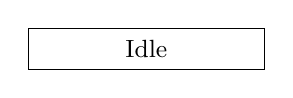
\begin{tikzpicture}
                \node (pubusy) [minimum width=30mm] {\small Idle};
            \end{tikzpicture}
        };
        \node[draw=black, thick, label=below:Channel 3] (channel3) [below=of channel2, yshift=-7.5mm] {
            
\begin{tikzpicture}
                \node (pubusy) [fill=green!20, minimum width=30mm] {\small Idle};
            \end{tikzpicture}
        };
        \node[draw=black, thick, label=below:Channel 4] (channel4) [below=of channel3, yshift=-7.5mm] {
            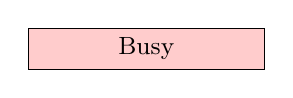
\begin{tikzpicture}
                \node (pubusy) [fill=red!20, minimum width=30mm] {\small Busy};
            \end{tikzpicture}
        };

        \node[draw] (mrcrn) [right=of channel3, yshift=0.8cm, xshift=0.25cm] {
            \begin{tikzpicture} [scale=0.625, transform shape]
            \node[draw=white, thick] (su2) [right=of channel3, xshift=1mm] {
            \begin{tikzpicture} [scale=0.5]
            \draw [line width=0.25mm, green!50!black] (2, -0.44) to (2.5,0.44);
            \draw [line width=0.25mm, green!50!black] (3, -0.44) to (2.5,0.44);
            \draw [line width=0.25mm, green!50!black] (2, -0.44) to (3,-0.44);
            \draw [line width=0.25mm, green!50!black] (2.5, -0.44) to (2.5,0.44);
            \draw [fill=green!50!black, green!50!black] (2.5,0.44) circle(1.5mm);

            \draw [line width=0.25mm, green!50!black] (2.5, 0.725) to (2.5,1.0);
            \draw [line width=0.25mm, green!50!black] (2.65, 0.65) to (2.825,0.85);
            \draw [line width=0.25mm, green!50!black] (2.725, 0.44) to (3,0.44);
            \draw [line width=0.25mm, green!50!black] (2.35, 0.65) to (2.175,0.85);
            \draw [line width=0.25mm, green!50!black] (2.275, 0.44) to (2,0.44);

            \end{tikzpicture}
        };

        

        \node[draw=white, thick] (su3) [right=of channel2, xshift=1mm] {
            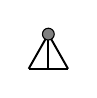
\begin{tikzpicture} [scale=0.5]
            \draw [line width=0.25mm] (2, -0.44) to (2.5,0.44);
            \draw [line width=0.25mm] (3, -0.44) to (2.5,0.44);
            \draw [line width=0.25mm] (2, -0.44) to (3,-0.44);
            \draw [line width=0.25mm] (2.5, -0.44) to (2.5,0.44);
            \draw [fill=gray] (2.5,0.44) circle(1.5mm);

            \end{tikzpicture}
        };
        
        \end{tikzpicture}
        };

        \node[draw=white, thick] (pu1) [left=of channel1, xshift=-1mm] {
            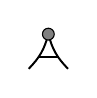
\begin{tikzpicture} [scale=0.5]
            \draw [line width=0.25mm, bend right = 15] (2, -0.44) to (2.5,0.44);
            \draw [line width=0.25mm, bend left = 15] (3, -0.44) to (2.5,0.44);
            \draw [line width=0.25mm] (2.25, -0.15) to (2.75,-0.15);
            %\draw [line width=0.25mm] (2.5, -0.44) to (2.5,0.44);
            \draw [fill=gray] (2.5,0.44) circle(1.5mm);

            \end{tikzpicture}
        };

        \node[draw=white, thick] (pu2) [left=of channel2, xshift=-1mm] {
            
\begin{tikzpicture} [scale=0.5]
            \draw [line width=0.25mm, bend right = 15, red] (2, -0.44) to (2.5,0.44);
            \draw [line width=0.25mm, bend left = 15, red] (3, -0.44) to (2.5,0.44);
            \draw [line width=0.25mm, red] (2.25, -0.15) to (2.75,-0.15);
            %\draw [line width=0.25mm] (2.5, -0.44) to (2.5,0.44);
            \draw [fill=red, red] (2.5,0.44) circle(1.5mm);

            \draw [line width=0.25mm, red] (2.5, 0.725) to (2.5,1.0);
            \draw [line width=0.25mm, red] (2.65, 0.65) to (2.825,0.85);
            \draw [line width=0.25mm, red] (2.725, 0.44) to (3,0.44);
            \draw [line width=0.25mm, red] (2.35, 0.65) to (2.175,0.85);
            \draw [line width=0.25mm, red] (2.275, 0.44) to (2,0.44);

            \end{tikzpicture}
        };

        \node[draw=white, thick] (pu3) [left=of channel3, xshift=-1mm] {
            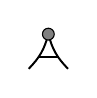
\begin{tikzpicture} [scale=0.5]
            \draw [line width=0.25mm, bend right = 15] (2, -0.44) to (2.5,0.44);
            \draw [line width=0.25mm, bend left = 15] (3, -0.44) to (2.5,0.44);
            \draw [line width=0.25mm] (2.25, -0.15) to (2.75,-0.15);
            %\draw [line width=0.25mm] (2.5, -0.44) to (2.5,0.44);
            \draw [fill=gray] (2.5,0.44) circle(1.5mm);

            \end{tikzpicture}
        };

        \node[draw=white, thick] (pu4) [left=of channel4, xshift=-1mm] {
            
\begin{tikzpicture} [scale=0.5]
            \draw [line width=0.25mm, bend right = 15, red] (2, -0.44) to (2.5,0.44);
            \draw [line width=0.25mm, bend left = 15, red] (3, -0.44) to (2.5,0.44);
            \draw [line width=0.25mm, red] (2.25, -0.15) to (2.75,-0.15);
            %\draw [line width=0.25mm] (2.5, -0.44) to (2.5,0.44);
            \draw [fill=red, red] (2.5,0.44) circle(1.5mm);

            \draw [line width=0.25mm, red] (2.5, 0.725) to (2.5,1.0);
            \draw [line width=0.25mm, red] (2.65, 0.65) to (2.825,0.85);
            \draw [line width=0.25mm, red] (2.725, 0.44) to (3,0.44);
            \draw [line width=0.25mm, red] (2.35, 0.65) to (2.175,0.85);
            \draw [line width=0.25mm, red] (2.275, 0.44) to (2,0.44);

            \end{tikzpicture}
        };
    \end{tikzpicture}
    \end{center}
    \end{minipage}\hfill
    \begin{minipage}[c][6cm][c]{\dimexpr0.5\textwidth-0.5\Colsep\relax}
    \begin{center}
    \begin{tikzpicture} [scale=1.0, transform shape]%show background rectangle,
        \tikzstyle{every node} = [draw, shape = rectangle, node distance=0mm, minimum width=5mm, minimum height=5.2mm]
        \node[draw=black, thick, label=below:Channel 2] (channel2) {
            \begin{tikzpicture}
                \node (puidle) [fill=green!20, minimum width=30mm] {\small Idle};%
            \end{tikzpicture}
        };
        \node[draw=black, thick, label=below:Channel 1] (channel1) [above=of channel2, yshift=7.5mm] {
            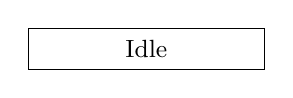
\begin{tikzpicture}
                \node (pubusy) [minimum width=30mm] {\small Idle};
            \end{tikzpicture}
        };
        \node[draw=black, thick, label=below:Channel 3] (channel3) [below=of channel2, yshift=-7.5mm] {
            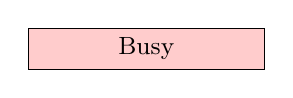
\begin{tikzpicture}
                \node (pubusy) [fill=red!20, minimum width=30mm] {\small Busy};
            \end{tikzpicture}
        };
        \node[draw=black, thick, label=below:Channel 4] (channel4) [below=of channel3, yshift=-7.5mm] {
            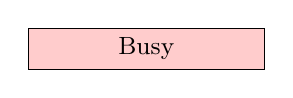
\begin{tikzpicture}
                \node (pubusy) [fill=red!20, minimum width=30mm] {\small Busy};
            \end{tikzpicture}
        };

        \node[draw] (mrcrn) [right=of channel3, yshift=0.8cm, xshift=0.25cm] {
            \begin{tikzpicture} [scale=0.625, transform shape]

        

        \node[draw=white, thick] (su2) [right=of channel3, xshift=1mm] {
            \begin{tikzpicture} [scale=0.5]
            \draw [line width=0.25mm] (2, -0.44) to (2.5,0.44);
            \draw [line width=0.25mm] (3, -0.44) to (2.5,0.44);
            \draw [line width=0.25mm] (2, -0.44) to (3,-0.44);
            \draw [line width=0.25mm] (2.5, -0.44) to (2.5,0.44);
            \draw [fill=gray] (2.5,0.44) circle(1.5mm);

            \end{tikzpicture}
        };

        \node[draw=white, thick] (su3) [right=of channel2, xshift=1mm] {
            
\begin{tikzpicture} [scale=0.5]
            \draw [line width=0.25mm, green!50!black] (2, -0.44) to (2.5,0.44);
            \draw [line width=0.25mm, green!50!black] (3, -0.44) to (2.5,0.44);
            \draw [line width=0.25mm, green!50!black] (2, -0.44) to (3,-0.44);
            \draw [line width=0.25mm, green!50!black] (2.5, -0.44) to (2.5,0.44);
            \draw [fill=green!50!black, green!50!black] (2.5,0.44) circle(1.5mm);

            \draw [line width=0.25mm, green!50!black] (2.5, 0.725) to (2.5,1.0);
            \draw [line width=0.25mm, green!50!black] (2.65, 0.65) to (2.825,0.85);
            \draw [line width=0.25mm, green!50!black] (2.725, 0.44) to (3,0.44);
            \draw [line width=0.25mm, green!50!black] (2.35, 0.65) to (2.175,0.85);
            \draw [line width=0.25mm, green!50!black] (2.275, 0.44) to (2,0.44);

            \end{tikzpicture}
        };
        \end{tikzpicture}
        };

        \node[draw=white, thick] (pu1) [left=of channel1, xshift=-1mm] {
            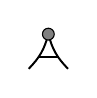
\begin{tikzpicture} [scale=0.5]
            \draw [line width=0.25mm, bend right = 15] (2, -0.44) to (2.5,0.44);
            \draw [line width=0.25mm, bend left = 15] (3, -0.44) to (2.5,0.44);
            \draw [line width=0.25mm] (2.25, -0.15) to (2.75,-0.15);
            %\draw [line width=0.25mm] (2.5, -0.44) to (2.5,0.44);
            \draw [fill=gray] (2.5,0.44) circle(1.5mm);

            \end{tikzpicture}
        };

        \node[draw=white, thick] (pu2) [left=of channel2, xshift=-1mm] {
            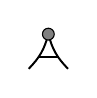
\begin{tikzpicture} [scale=0.5]
            \draw [line width=0.25mm, bend right = 15] (2, -0.44) to (2.5,0.44);
            \draw [line width=0.25mm, bend left = 15] (3, -0.44) to (2.5,0.44);
            \draw [line width=0.25mm] (2.25, -0.15) to (2.75,-0.15);
            %\draw [line width=0.25mm] (2.5, -0.44) to (2.5,0.44);
            \draw [fill=gray] (2.5,0.44) circle(1.5mm);

            \end{tikzpicture}
        };

        \node[draw=white, thick] (pu3) [left=of channel3, xshift=-1mm] {
            
\begin{tikzpicture} [scale=0.5]
            \draw [line width=0.25mm, bend right = 15, red] (2, -0.44) to (2.5,0.44);
            \draw [line width=0.25mm, bend left = 15, red] (3, -0.44) to (2.5,0.44);
            \draw [line width=0.25mm, red] (2.25, -0.15) to (2.75,-0.15);
            %\draw [line width=0.25mm] (2.5, -0.44) to (2.5,0.44);
            \draw [fill=red, red] (2.5,0.44) circle(1.5mm);

            \draw [line width=0.25mm, red] (2.5, 0.725) to (2.5,1.0);
            \draw [line width=0.25mm, red] (2.65, 0.65) to (2.825,0.85);
            \draw [line width=0.25mm, red] (2.725, 0.44) to (3,0.44);
            \draw [line width=0.25mm, red] (2.35, 0.65) to (2.175,0.85);
            \draw [line width=0.25mm, red] (2.275, 0.44) to (2,0.44);

            \end{tikzpicture}
        };

        \node[draw=white, thick] (pu4) [left=of channel4, xshift=-1mm] {
            
\begin{tikzpicture} [scale=0.5]
            \draw [line width=0.25mm, bend right = 15, red] (2, -0.44) to (2.5,0.44);
            \draw [line width=0.25mm, bend left = 15, red] (3, -0.44) to (2.5,0.44);
            \draw [line width=0.25mm, red] (2.25, -0.15) to (2.75,-0.15);
            %\draw [line width=0.25mm] (2.5, -0.44) to (2.5,0.44);
            \draw [fill=red, red] (2.5,0.44) circle(1.5mm);

            \draw [line width=0.25mm, red] (2.5, 0.725) to (2.5,1.0);
            \draw [line width=0.25mm, red] (2.65, 0.65) to (2.825,0.85);
            \draw [line width=0.25mm, red] (2.725, 0.44) to (3,0.44);
            \draw [line width=0.25mm, red] (2.35, 0.65) to (2.175,0.85);
            \draw [line width=0.25mm, red] (2.275, 0.44) to (2,0.44);

            \end{tikzpicture}
        };
    \end{tikzpicture}
    \end{center}
    \end{minipage}%
\end{minipage}
